\documentclass[12pt, a4paper]{article}
\usepackage{graphicx}
\usepackage{pgfplots}
\usepackage{mathtools}
\usepackage{fancyhdr}
\usepackage{multicol}
\usepackage{cancel}
\usepackage{geometry}
\usepackage{listings}
\usepackage{booktabs}
\usepackage{tabularx}
\usepackage{subfig}
\usepackage{hyperref}
\usepackage{float}
\usepackage{titlesec}
\usepackage{tikz, pgfplots}
\usepackage[utf8]{inputenc}
\usepackage[backend=bibtex8,style=ieee]{biblatex}

% Requirement libs
\usetikzlibrary{positioning}

% Options
\nonstopmode % To make sure that you dont have to press input for each error
\geometry{top=1in, left = 1in, right = 1in, bottom=1.2in}
\pgfplotsset{compat=1.18}
\graphicspath{{./figures/}}
\setlength{\columnsep}{0.7cm}

% Metadata
\addbibresource{./citations.bib}
\author{Aris Podotas}
\date{today}

% Herlink setup
\hypersetup{
    colorlinks=true,
    linkcolor=blue,
    filecolor=magenta,
    urlcolor=cyan,
    pdftitle={MLICB Assignment 1},
    pdfpagemode=FullScreen,
}

% For the code blocks
\definecolor{codegreen}{rgb}{0.03,0.5,0.03}
\definecolor{codegray}{rgb}{0.5,0.5,0.5}
\definecolor{codepurple}{rgb}{0.58,0,0.82}
\definecolor{backcolour}{rgb}{0.95,0.95,0.95}

% Code block setup
\lstdefinestyle{mystyle}{
    backgroundcolor=\color{backcolour},
    commentstyle=\color{codegreen},
    keywordstyle=\color{magenta},
    numberstyle=\tiny\color{codegray},
    stringstyle=\color{codepurple},
    basicstyle=\ttfamily\footnotesize,
    breakatwhitespace=false,
    breaklines=true,
    captionpos=b,
    keepspaces=true,
    numbers=left,
    numbersep=5pt,
    showspaces=false,
    showstringspaces=false,
    showtabs=false,
    tabsize=4,
    escapeinside = {(*}{*)}
}
\lstset{style=mystyle}

% My custom headers and margins 
\pagestyle{fancy}
\setlength{\headheight}{44pt}
\setlength{\headsep}{18pt}
\lhead{\includegraphics[scale = 0.2]{~/Documents/Masters/bnw unit.png}}
\chead{\quad Data Science and Information Technologies Master’s
National and Kapodistrian University of Athens}
\rhead{}
\lfoot{}
\cfoot{\thepage}
\rfoot{}

% Start
\begin{document}

% Custom title page
\begin{titlepage}
    \centering
    {\huge \textbf{Assignment 2}\par}
    \vspace{0.5cm}
    {\Large \textbf{Name:} Aris Podotas\par}
    \vspace{0.5cm}
    {\large \textbf{University:} National and Kapodistrian University of Athens\par}
    \vspace{0.5cm}
    {\large \textbf{Program:} Data Science and Information Technologies\par}
    \vspace{0.5cm}
    {\large \textbf{Specialization:} Bioinformatics - Biomedical Data\par}
    \vspace{0.5cm}
    {\large \textbf{Lesson:} Image Processing \& analysis \par}
    \vspace{0.5cm}
    {\large \textbf{Date:} May 2025\par}
    \tableofcontents
\end{titlepage}

\begin{multicols}{2}

    \section{Exercise 1} \label{sec:ex1}

    The function is a step function that increases the output values by a variable amount with step $30$. The minimum intensity is $10$ and the maximum is $200$ which is less than the input range on both ends. This should generally dim the image to some degree. Let us compare this function to one that does not alter the image.
    \newline

\end{multicols}

\begin{figure}[H]
    \begin{center}
        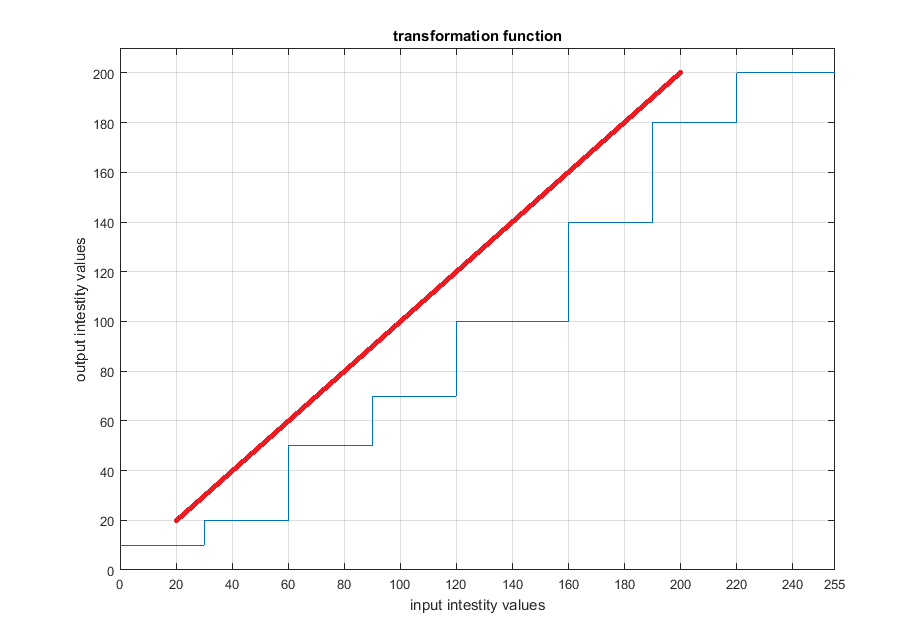
\includegraphics[width=0.95\textwidth]{figures/step_fun_vs_y_eq_x.png}
    \end{center}
    \caption{Comparison of the given function to one that does not alter the image (in red)}\label{fig:funcCompare}
\end{figure}

\begin{multicols}{2}

    Here we can see the dimming effect considering the step function is \textit{almost} always under the $y = x$ function that does not alter the image.
    \newline

    Since the function assigns an input range to a singular value we can expect some quantization of the output images. This should leave the output looking like a lower quality image and it will also be easier to compress but it will also be the same resolution right after the transformation.
    \newline

    \subsection{Example} \label{subsec:example}

    You can find the files that perform this transformation \href{./src/}{here}.
    \newline

\end{multicols}

\begin{figure}[H]
    \begin{center}
        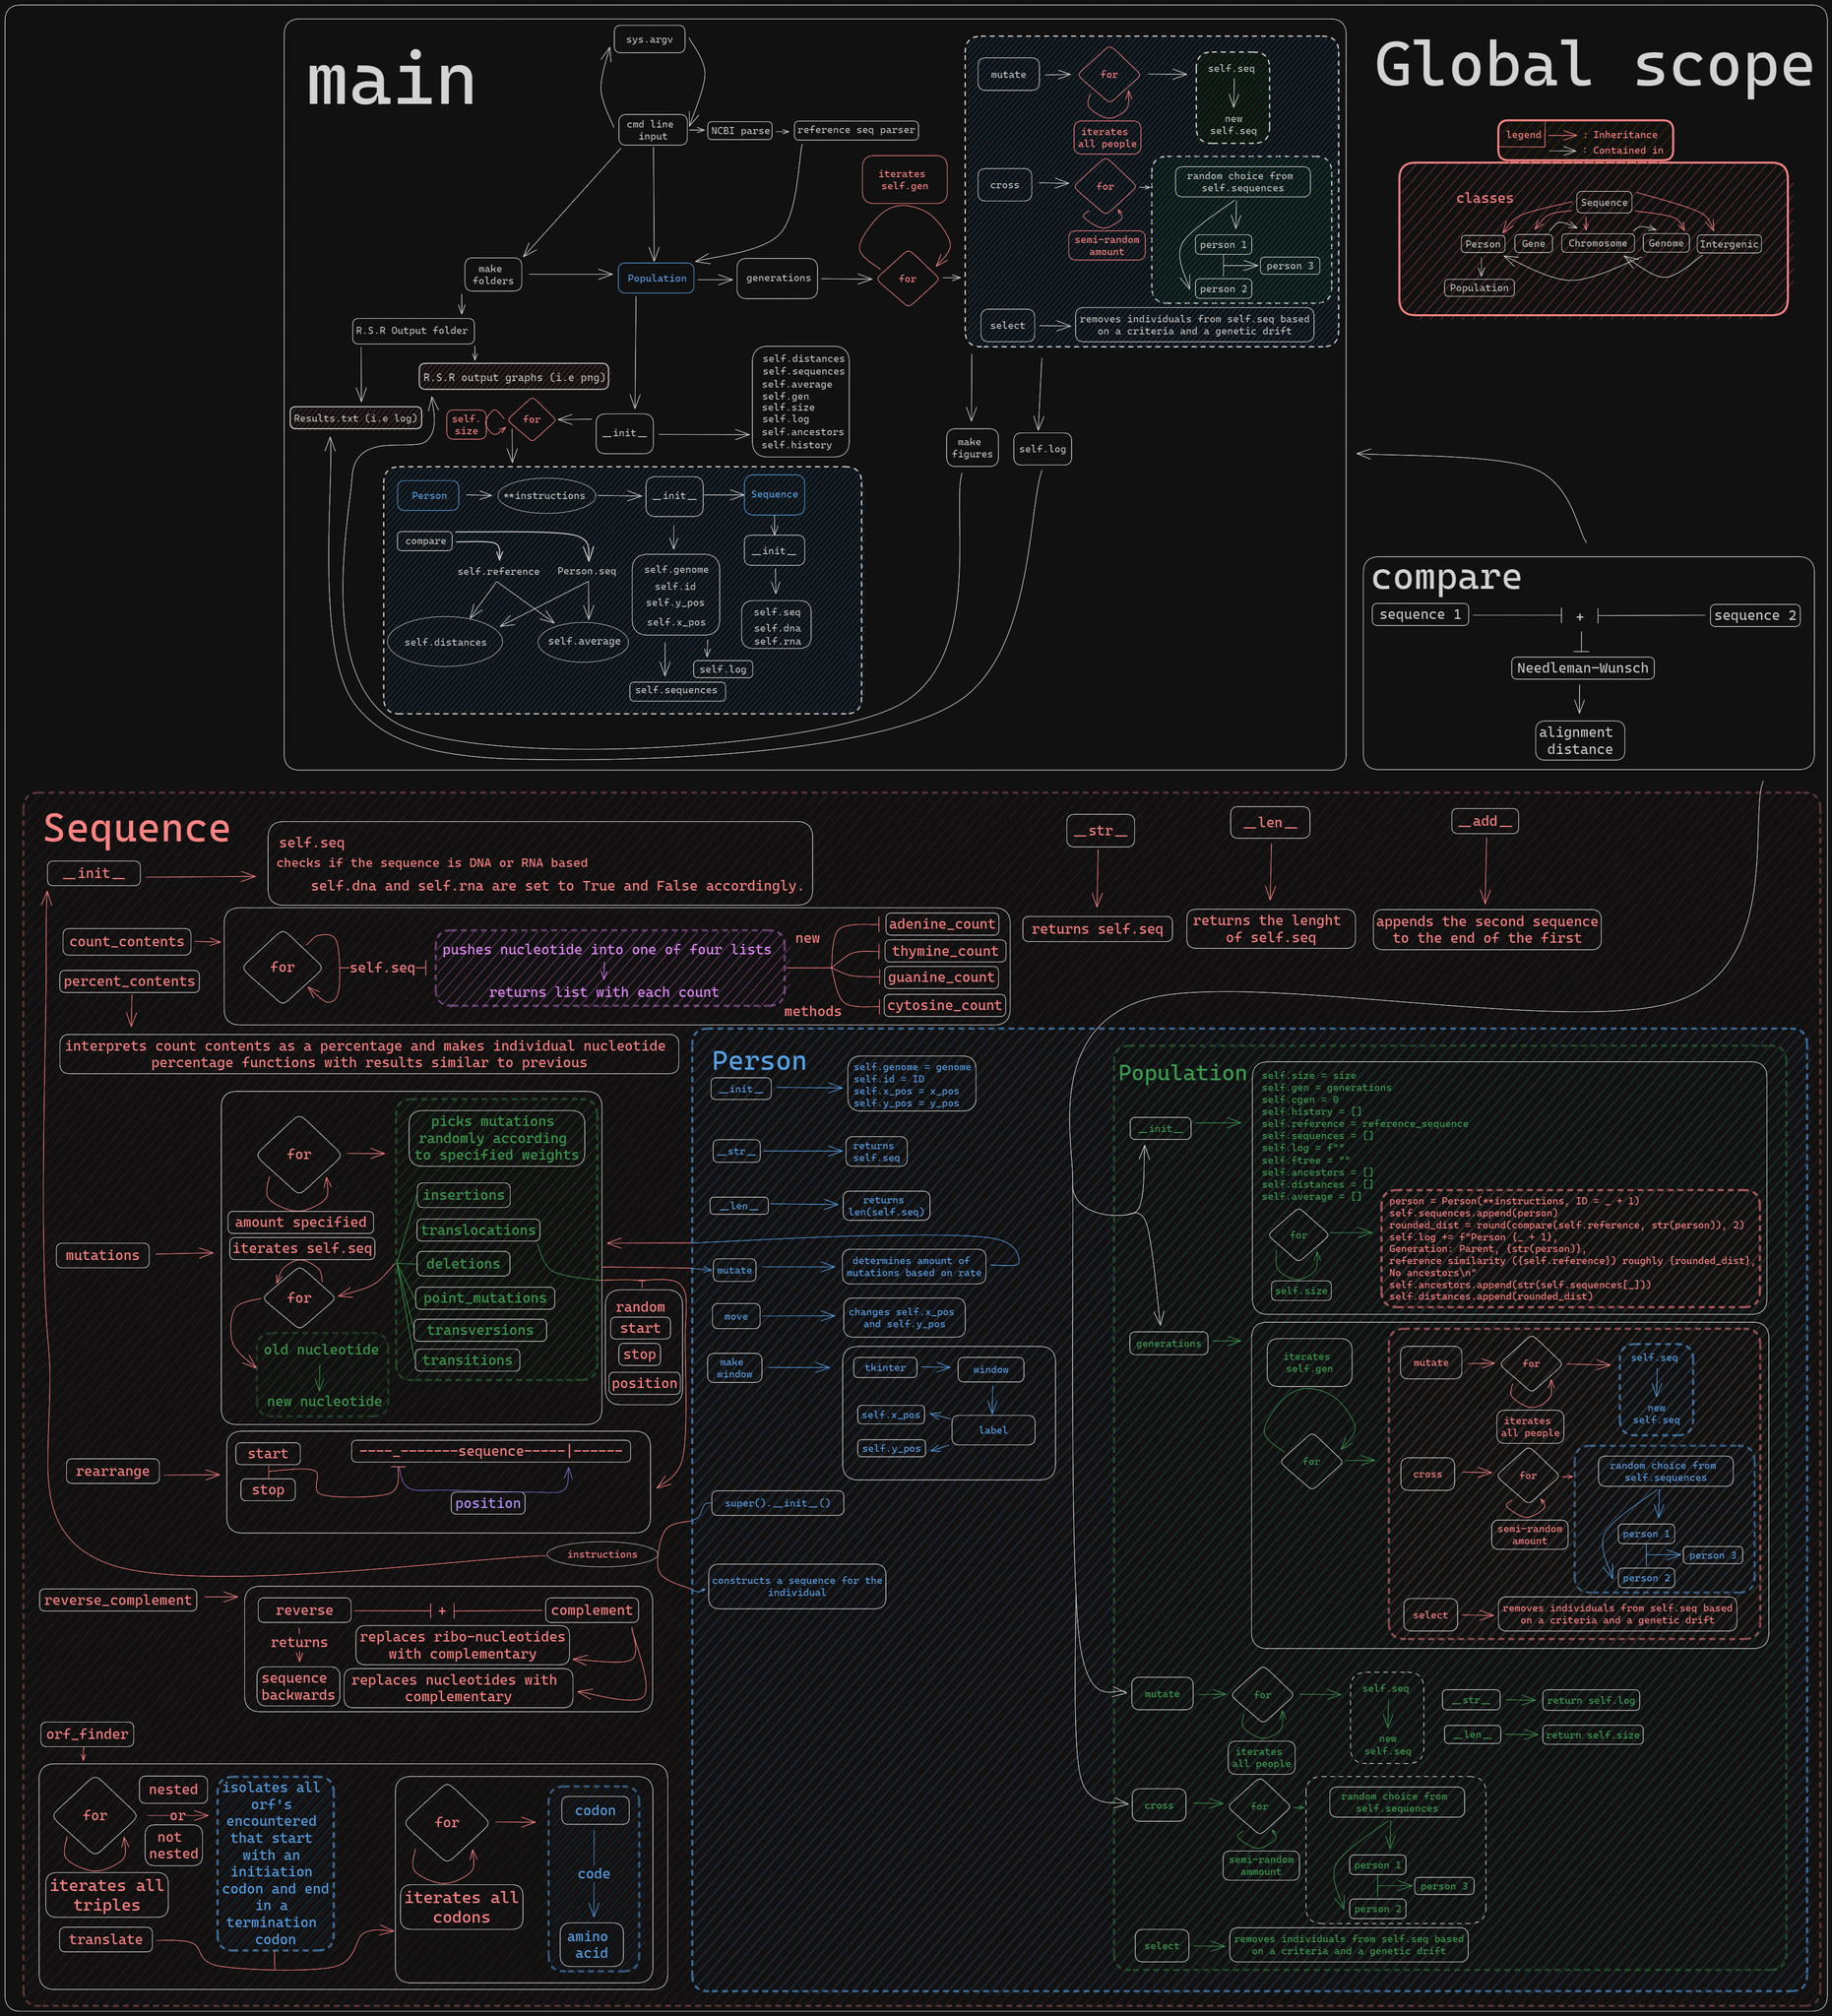
\includegraphics[width=0.95\textwidth]{figures/first requirement before.png}
    \end{center}
    \caption{Our image before the transformation}\label{fig:before}
\end{figure}

\begin{figure}[H]
    \begin{center}
        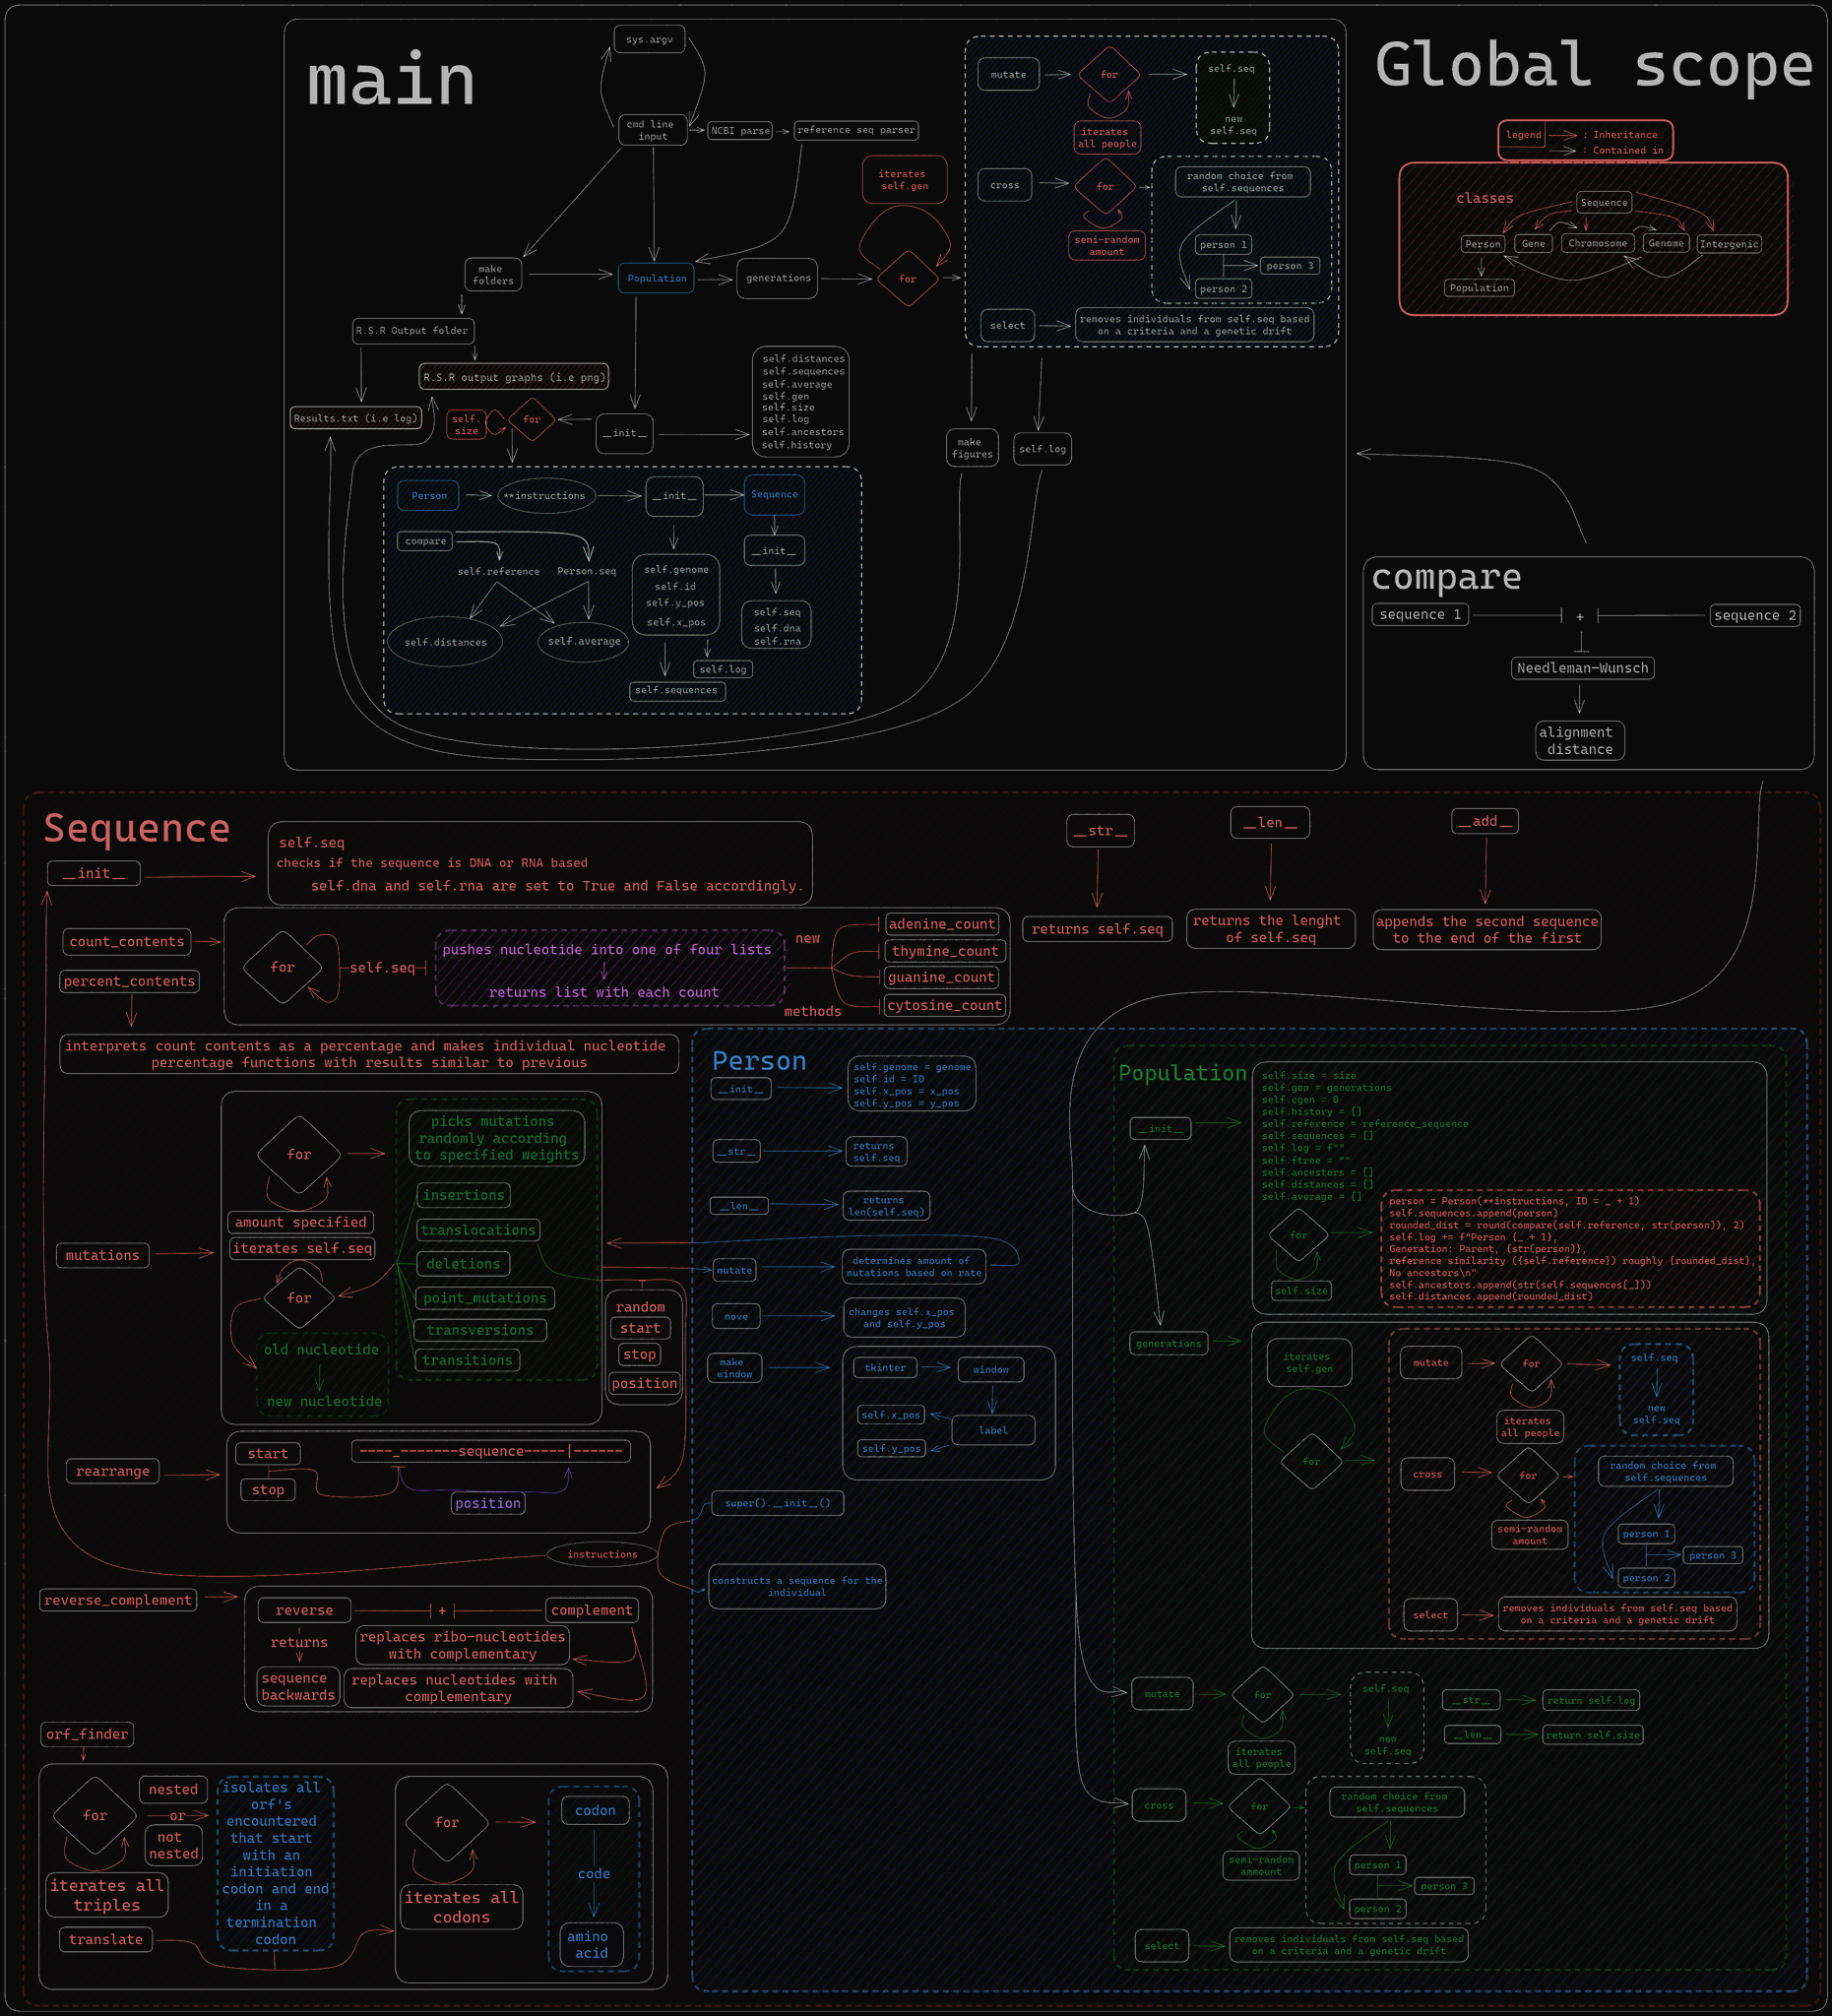
\includegraphics[width=0.95\textwidth]{figures/first requirement after.png}
    \end{center}
    \caption{Image after the transformation}\label{fig:after}
\end{figure}

\begin{multicols}{2}

    \begin{table}[H]
        \caption{Comparison of Images}\label{tab:comp}
        \begin{center}
            \resizebox{0.45 \textwidth}{!}{
                \begin{tabular}[c]{l|l|l|}
                    \hline
                    \multicolumn{1}{c|}{\textbf{Image}} & 
                    \multicolumn{1}{c}{\textbf{File Size (disk)}} &
                    \multicolumn{1}{c}{\textbf{Shape}} \\
                    \hline
                    Before & $3.29$ MB & $1861 \times 2048$ \\
                    After & $652$ KB & $1861 \times 2048$ \\
                    \hline
                \end{tabular}
            }
        \end{center}
    \end{table}

    We can see the quantization into a lower quality image while maintaining the same dimensions but a much lower disk space.
    \newline

    \section{Exercise 2} \label{sec:ex2}
    \section{Exercise 3} \label{sec:ex3}
    \section{Exercise 4} \label{sec:ex4}
    \section{Exercise 5} \label{sec:ex5}
    \section{Exercise 6} \label{sec:ex6}
    \section{Exercise 7} \label{sec:ex7}

    \printbibliography

\end{multicols}

\end{document}

